% begin module polar-area-ex1
\begin{frame}
\begin{example} %[Example 1, p. 686]
Find the area enclosed by one loop of the four-leaved rose $r = \cos 2\theta$.
\begin{columns}[T]
\column{.5\textwidth}
\psset{xunit=2cm, yunit=2cm, algebraic=true}
\begin{pspicture}(-1.25,-1.25)(1.25,1.25)
\tiny%
\fcBoundingBox{-1.25}{-1.25}{1.25}{1.25}
\uncover<2->{%
\pscustom*[linecolor=\fcColorAreaUnderGraph]{%
\parametricplot{-0.785398163}{0.785398163}{cos(2*t)*cos(t)|cos(2*t)*sin(t)}%
}%
\rput(-0.8,0.8){$r=\cos (2\theta)$}
\parametricplot[linecolor=\fcColorGraph, plotpoints=1000] {0}{6.283185307}{cos(2*t)*cos(t)|cos(2*t)*sin(t)}%
}
\fcAxesStandardNoFrame{-1.2}{-1.2}{1.2}{1.2}%
\uncover<3->{
\psline[linecolor=\fcColorTangent](0,0)(1.2,1.2)
\psline[linecolor=\fcColorTangent](0,0)(1.2,-1.2)
\rput[r](1, 1.1){$\theta=\frac{\pi}{4}$}
\rput[r](1, -1.1){$\theta=-\frac{\pi}{4}$}
}
\end{pspicture}
%\ \uncover<2->{%
%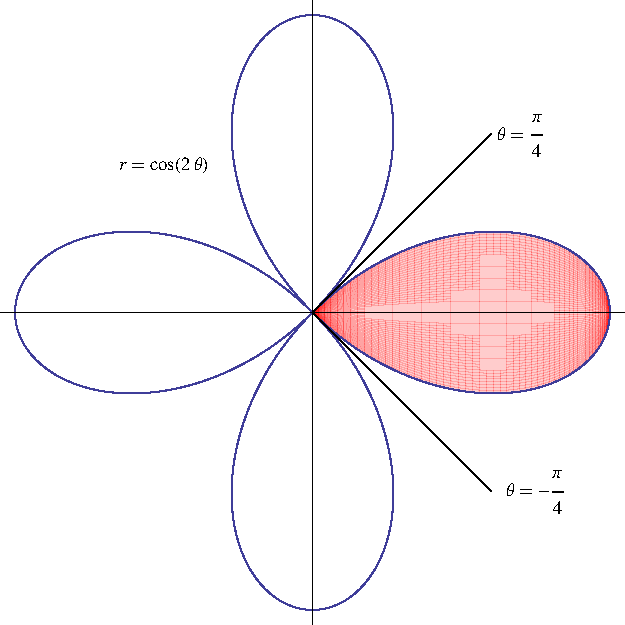
\includegraphics[height=5cm]{polar-curves/pictures/11-04-ex1a.pdf}%
%}%

\uncover<2->{%
The region enclosed by the right loop corresponds to points whose  \alertNoH{2,3}{$\theta$ polar coordinate lies in the interval} $\uncover<3->{ \alertNoH{3,4}{ -\frac{\pi}{4}}} \alertNoH{2,3,4}{\leq \theta \leq } \fcAnswer{3}{\alertNoH{4}{\frac{\pi}{4}}} $.
}%
\column{.5\textwidth}
\begin{eqnarray*}
\uncover<4->{%
A%
}%
& \uncover<4->{ = } &%
\uncover<4->{%
\int_{\alertNoH{4}{-\frac{\pi}{4}} }^{\alertNoH{4}{\frac{\pi} {4} }}\frac{1}{2}\alertNoH{5}{r^2}\diff \theta%
}\\%
& \uncover<5->{ = } &%
\uncover<5->{%
\alertNoH{ 6}{\frac{1}{2}} \int_{\alertNoH{ 6}{-\frac{\pi}{4}}}^{\alertNoH{ 6}{\frac{\pi}{4}}}\alertNoH{ 5}{\cos^2(2\theta)} \diff \theta%
}\\%
& \uncover<6->{ = } &%
\uncover<6->{%
\int_{\alertNoH{ 6}{0}}^{\alertNoH{ 6}{\frac{\pi}{4}}}\alertNoH{ 7}{\cos^2(2\theta)} \diff \theta%
}\\%
& \uncover<7->{ = } &%
\uncover<7->{%
\int_{0}^{\frac{\pi}{4}}\alertNoH{ 7}{\frac{1}{2}(1+\cos (4\theta) )}\diff \theta%
}\\%
& \uncover<8->{ = } &%
\uncover<8->{%
\frac{1}{2}\left[ \theta + \frac{1}{4}\sin (4\theta) \right]_0^{\frac{\pi}{4}}%
}\\%
& \uncover<9->{ = } &%
\uncover<9->{%
\frac{\pi}{8}%
}%
\end{eqnarray*}
\end{columns}
\end{example}
\end{frame}
% end module polar-area-ex1
